\section{Vordefiniertes Stylesheet}

Das vordefinierte Stylesheet befindet sich im Ordner default unter Packages. Auf diesem Stylesheet aufbauend, wird die Beschreibung von Quests und Packages, welche keine eigene style.css beinhalten, verwenet.

Diese ist vorallem für bestimmte Anwendungsgebiete zugeschnitten:
\begin{itemize}
\item Um Codes zu kennzeichen kann der die Klasse \textit{\textbf{code}} verwendet werden. Diese Umrahmt die Auswahl mit gepunkteten Linien.
\item Informationen werden mit der Klasse \textit{\textbf{info}} gekenzeichnet und diese werden mit einer gelben Hintergrundfarbe dargestellt.
\item Fragen haben einen blauen Hintergrund, und werden mithilfe der Klasse \textit{\textbf{question}} angesprochen.
\item Duch einen roten Hintergrund kann eine Warnung dargestellt werden. Diese kann anhand der Klasse \textit{\textbf{warning}} verwendet werden.
\end{itemize}

\begin{figure}[h] 
  \centering
     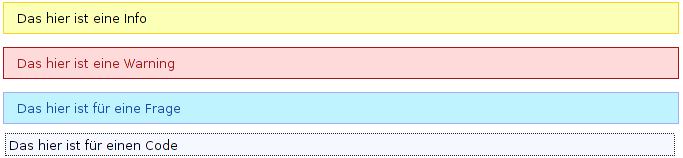
\includegraphics[width=1\textwidth]{./media/images/quest/style.png}
  \caption{Standart Stylesheet Infos}
  \label{fig:defaut_stylesheet}
\end{figure}